\documentclass{ltxdoc} % Process with xelatex -shell-escape
\usepackage[verbose,unique]{bashful}

\usepackage[colorlinks=true]{hyperref}
\usepackage{gensymb}
\usepackage{graphicx}
\usepackage{metalogo}
\usepackage{xkvview}
\usepackage{xspace}
\usepackage{amsmath}
\usepackage{multicol}

\newcommand\me{bashful}
\newcommand\bashful{\textsf{\me}\xspace}
\lstdefinestyle{input}{basicstyle=\ttfamily\footnotesize,
    keywords={},upquote=true,extendedchars=false,
    showstringspaces=false,aboveskip=0pt,belowskip=0pt}
\lstdefinestyle{scriptsize}{style=input,basicstyle=\ttfamily\scriptsize}

% listings style for the script, standard output file, and standard error file. 
\lstdefinestyle{bashfulScript}{style=input}
\lstdefinestyle{bashfulStdout}{style=input}
\lstdefinestyle{bashfulStderr}{style=input,
  basicstyle=\ttfamily\footnotesize\color{red}}
\newcommand\listFile[1]{%
  \vspace{0.8em plus 0.3em minus 0.3em}%
  \lstinputlisting[style=input,frameround=ftttt,frame=trBL]{#1}%
  \vspace{0.8em plus 0.3em minus 0.3em}}

\title{The \bashful Package\thanks{
   Copyright \copyright{} 2011, 2012 by Yossi Gil  
    \url{mailto:yogi@cs.technion.ac.il}.
  This work may be distributed and/or modified under the conditions of the
    \emph{\LaTeX{} Project Public License} (LPPL), either version 1.3 of this 
    license or (at your option) any later version.  
The latest version of this license is in 
  \url{http://www.latex-project.org/lppl.txt} and version 1.3 or later 
  is part of all distributions of \LaTeX{} version 2005/12/01 or later.
This work has the LPPL maintenance status `maintained'.
The Current Maintainer of this work is Yossi Gil. 
This work consists of the files \texttt{\me.tex} and \texttt{\me.sty} 
  and the derived file
  \texttt{\me.pdf}
}}

\author{Yossi Gil\thanks{\url{mailto:yogi@cs.Technion.ac.IL}}\\
   \normalsize Department of Computer Science\\
   \normalsize The Technion---Israel Institute of Technology\\
   \normalsize Technion City, Haifa 32000, Israel
}

\makeatletter
\date{\date@bashful\thanks{
      This document describes \bashful \version@bashful.}}
\makeatother

\begin{document}
\bash
cat << EOF > README
The bashful package, v 0.93

This package makes it possible to execute bash scripts from within LaTeX. The
main application is in writing computer-science texts, in which you want to
make sure the programs listed in the document are executed directly from the
input. 

This package may be distributed and/or modified under the LaTeX Project Public
License, version 1.3 or higher (your choice). The latest version of this
license is at: http://www.latex-project.org/lppl.txt

This work is author-maintained (as per LPPL maintenance status)
by Yossi Gil, <yogi@cs.Technion.ac.i>
EOF
\END

\bash[verbose,stdoutFile=bashful.date]
stat -c %y bashful.sty | sed -e s+-+/+g -e 's/ .*//g' > date
\END

\maketitle

\begin{abstract}
\parindent 1.5ex
\parskip 0.5em

\sl
It is sometimes useful to ``\emph{escape-to-shell}'' from within
  \LaTeX{}. 
The most obvious application is when the document
  explains something about the working of a computer program.
Your text would be more robust to changes, and easier to write,
  if all the examples it gives, are run directly from
  within \LaTeX{}.
  
To facilitate this and other applications, 
  package \bashful{} provides a convenient interface to \TeX's 
  primitive \verb+\write18+---the execution of shell commands from within
  your input files, also known as \emph{shell escape}. 
Text between \verb+\bash+ and \verb+\END+ is executed by 
   \href
        {http://en.wikipedia.org/wiki/Bash_%28Unix_shell%29}
        {\texttt{bash}},
  a popular Unix command line interpreter.
Various flags control whether the executed commands and their output 
  show up in the printed document, and whether they are saved
  to files. 

Although provisions are made for using shells other 
  than \texttt{bash}, this package may \emph{not} operate without
  modifications on  Microsoft's operating systems.
\end{abstract}

\begin{multicols}{2}
\footnotesize 
\tableofcontents
\end{multicols}

\parindent 1.5ex
\parskip 0.5em

\section{Introduction}

\bash[verbose,scriptFile=temperature.sh,stdoutFile=temperature.tex]
location=Jerusalem,Israel
server="http://www.Google.com/ig/api"
request="$server?weather=$location" 
wget -q -O - $request |\
tr "<>" "\012\012" |\
grep temp_c |\
sed 's/[^0-9]//g'
\END

\bash[verbose,scriptFile=condition.sh,stdoutFile=condition.tex]
location=Jerusalem,Israel
server="http://www.Google.com/ig/api"
request="$server?weather=$location" 
wget -q -O - $request |\
tr "<>" "\012\012" |\
grep "condition data" |\
head -n 1 |\ 
sed -e 's/^.*="//' -e 's/"\/*//' |\
tr 'A-Z' 'a-z'
\END

At the time I run this document through \LaTeX{}, 
  the temperature in Jerusalem, Israel, 
  was~\emph{\input{temperature}\unskip\celsius}, 
  while the weather condition was 
  \emph{\input{condition}}\unskip.
  
You may not care so much about these bits of truly
  ephemeral information,
  but you may be surprised that they were produced 
  by the very process of \LaTeX{}ing the input.

\bash
cat << EOF > ls.tex
\documentclass{article}
\usepackage[a6paper]{geometry}
\usepackage{bashful}
\pagestyle{empty}
\begin{document}
The directories in my \texttt{/usr} directory are: 
\bash[stdout]
ls -F /usr
EOF
echo "\\END" >> ls.tex
cat << EOF >> ls.tex
That's it!
\end{document}
EOF
xelatex -shell-escape ls.tex
\END

Before I tell you how I generated this information, 
	let me demonstrate the use of the \bashful package for the purpose of
	incorporating the list of files in a folder into your output. 

This simple \LaTeX{} file generates a listing of all files
  in the \texttt{/usr} directory, using the UNIX \texttt{ls}
  command:

\begin{minipage}{\textwidth}
\listFile{ls.tex}
\end{minipage}

The printed output of this file is then

\begin{center}
  \fbox{\includegraphics[scale=0.8,trim=20 200 40 50]{ls.pdf}}
\end{center}

To generate the weather information, I wrote 
  a series of shell commands that retrieve the current temperature,
  and another such series to obtain the current 
  weather conditions.  
This task required connection to 
  \href{http://www.Google.com/support/forum/p/%
        apps-apis/thread?tid=0c95e45bd80def1a&hl=en}%
  {Google's weather service} and 
  minimal dexterity with Unix pipes and filters to process the output.
  
My command series to obtain the current temperature was:
 
\begin{minipage}{\textwidth}
\begin{quote}
  \lstinputlisting[style=input]{temperature.sh}
\end{quote}
\end{minipage}

while the weather condition was obtained by 

\begin{minipage}{\textwidth}
\begin{quote}
  \lstinputlisting[style=input]{condition.sh}
\end{quote}
\end{minipage}

The second step was coercing \LaTeX{} to run these commands
  while processing my document.  
To do that, I used package \bashful,
\begin{verbatim}
\usepackage{bashful}
\end{verbatim}
And, then, I wrapped each of these two series within 
  a \verb+\bash+\ldots\verb+\END+ pair.
  
The \verb+\bash+ command, offered by this package,
  takes all subsequent lines, stopping at  the closing \verb+\END+,
  places these in a file, and then 
  lets the \texttt{bash} shell interpreter execute this file.

Allowing \LaTeX{} to run arbitrary shell commands can be 
  dangerous---you never know whether that nice looking \texttt{.tex}
  file you received by email was prepared by a friend or 
  a foe.
This is the reason that you have to tell \LaTeX{} 
  explicitly that shell escapes 
  are allowed. 
The \texttt{-shell-esc} flag does that.
To process my document, I typed, at the command line,
\begin{quote}
  \tt
  \% latex -shell-escape \jobname.tex
\end{quote}

What I actually wrote in the input 
  to produce the temperature in 
  Jerusalem, Israel was: 
  
\begin{minipage}{\textwidth}
\begin{quote}
\noindent\verb+\bash[verbose,scriptFile=temperature.sh,stdoutFile=temperature.tex]+
\lstinputlisting[style=input,belowskip=0pt]{temperature.sh}
\verb+\END+\\
\end{quote}
\end{minipage}

The flags passed to the \verb+bash+ control sequence above instructed it:
  \begin{enumerate}
    \item to be verbose, typing out a detailed log of everything it did;
    \item to save the shell commands in a script file named 
          \texttt{temperature.sh}; and,
    \item to store the standard output of the script in a file named 
          \texttt{temperature.tex}. 
  \end{enumerate}

To obtain the current weather condition in the capital I wrote: 

\begin{minipage}{\textwidth}
\begin{quote}
\noindent\verb+\bash[verbose,scriptFile=condition.sh,stdoutFile=condition.tex]+
\lstinputlisting[style=input]{condition.sh}
\verb+\END+
\end{quote}
\end{minipage}

I wrote these two just after my \verb+\begin{document}+. 
When \LaTeX{} encountered these, it executed the bash commands and 
  created two files \texttt{temperature.tex} and \texttt{condition.tex}.

Subsequently, I could use the content of these files by writing:

\begin{quote}
\bash
sed -n "/^At the time/,/^You may not/ p" bashful.tex  > init.tex
\END

\lstinputlisting[style=input,belowskip=0pt]{init.tex}\ldots
\end{quote}

\section{Application for Teaching Programming}
\bashful primary application is for writing documents which describe 
	computer programming.
You can include the programs in your text, and have them compiled
	and executed as part of the \LaTeX{} processing. 
To demonstrated I will first tell a simple story
  of writing, compiling and executing and 
    a short program.
Then, I will explain how I used the \verb+\bash+
  command to not only tell the story, but
  also to play it live: that is, authoring
  a simple~C program, compiling it and executing
  it, all from within \LaTeX{}.
  
\subsection{A ``Hello, World'' Program} 
 
\subsubsection{Authoring}
Let's first write a simple 
  \href{http://en.wikipedia.org/wiki/Hello_world_program}
    {Hello, World!} program in the 
    \href{http://en.wikipedia.org/wiki/C_(programming_language)}
    {C programming language}:


\bash[verbose,environment=quote,script]
rm -f hello.c; cat << EOF > hello.c
/* 
** hello.c: My first C program; it prints 
** "Hello, World!", and dies.
*/

#include <stdio.h> 

int main() 
{
  printf("Hello, World!\n");
  return 0;
}
EOF
\END

\subsubsection{Compiling}
Now, let's compile this program:
\bash[environment=quote,script,stdout]
cc hello.c
\END

\subsubsection{Executing}
Finally, we can execute this program,
  and see that indeed, it prints the ``Hello, World!''
  string.
\bash[environment=quote,script,stdout]
./a.out
\END


\subsection{Behind the Scenes}
\subsubsection{Authoring}
What I wrote in the input to produce the 
  \texttt{hello.c} program was:
  
\begin{minipage}{\textwidth}
\begin{quote}
\begin{verbatim}
\bash[script]
rm -f hello.c; cat << EOF > hello.c
/* 
** hello.c: My first C program; it prints 
** "Hello, World!", and dies.
*/

#include <stdio.h> 

int main() 
{
  printf("Hello, World!\n");
  return 0;
}
EOF
\END
\end{verbatim}
\end{quote}
\end{minipage}

In doing so, all the text between the \verb+\bash+
  and \verb+\END+ was sent to a temporary file,
    which was then sent for execution.
The \texttt{script} flag instructed \verb+\bash+
  to list this file in the main document.
This listing was prefixed with \verb*+% +
  to make it clear that it was input to \texttt{bash}.
 
\subsubsection{Compiling} 
Next, I wrote
\begin{quote}
\begin{verbatim}
\bash[script,stdout]
cc hello.c
\END
\end{verbatim}
\end{quote}

As before, in doing that, I achieved two objectives:
  first, when \LaTeX{} processed
  the input, it also invokes the~C compiler to compile
  file \texttt{hello.c}, the file which I just created.
  
Second, thanks to the \texttt{script} flag,
  the command for compiling this program
  was included in the printed version of 
  this document.
The \texttt{stdout} option instructed \verb+\bash+
 to include plain messages, i.e., not error messages,
 produced by the compiler in
  the printed version of this document.
In this case, no such messages were produced.


\subsubsection{Executing}

Finally, I wrote 
\begin{quote}
\begin{verbatim}
\bash[script,stdout]
./a.out
\END
\end{verbatim}
\end{quote}
to run the program I just wrote.
The \texttt{stdout} adds to my listing
  the output that this execution produces, i.e.,
  the string \texttt{Hello, World!} that this
  execution produces to the standard output.
  
\section{Dealing With Errors}
Using \bashful{} to demonstrate
  my \emph{Hello, World!} program, made
  sure that the story I told is accurate:
I really did everything I said I did.
More accurately, the \verb+\bash+ command
  acted as my proxy, and did it for me.
  
Luckily, my \texttt{hello.c} program was 
  correct.
But, if it was not, the \verb+\bash+ command would have detected
  the error, and would have stopped the \LaTeX{} process, 
  indicating that the compilation did not succeed.
More specifically, the \verb+\bash+ command 
\begin{enumerate}
\item collects all commands up to \verb+\END+; 
\item places these commands in a script file; 
\item change directory to a designated directory if the \texttt{hide}
    option is set (the \texttt{dir} option sets the directory name);
\item executes this script file, redirecting its standard output
      and its standard error streams to distinct files; 
\item checks whether the exit code of the execution indicates an error
  (i.e., exit code which is different from~$0$), and if so,
    place this exit code in a distinct file;
\item checks whether the file containing the standard error is empty,
    and if not, pauses execution after displaying an error message;
\item checks whether the file containing the exit code is empty,
    and if not, pauses execution after displaying an error message;
\item lists, if requested to, the script file;
\item lists, if requested to, the file containing the standard output; and,
\item lists, if requested to, the file containing the standard error;
\end{enumerate}

Let me demonstrate a situation in which the execution of 
  the script generates an error.
To do that, I will write a short \LaTeX{} file, named \texttt{minimal.tex}
  which tries to use \verb+\bash+ to compile an incorrect~C program.
Since \texttt{minimal.tex} contains \verb+\END+,
  I will have to author this file in three steps:
\begin{enumerate}
\item Creating the header of \texttt{minimal.tex}:
\bash[script]
cat << EOF > minimal.tex
\documentclass{article}
\usepackage[a6paper]{geometry}
\usepackage{bashful}
\pagestyle{empty}
\begin{document}
This document creates a simple erroneous C program
  and then compiles it:
\bash[script,stdout]
echo "main(){return int;}" > error.c
cc error.c
EOF
\END
\item Adding \verb+\END+ to \texttt{minimal.tex}
\bash[script]
echo "\\END" >> minimal.tex
\END
\item Finalizing \texttt{minimal.tex}
\bash[script]
echo "\\end{document}" >> minimal.tex
\END
\end{enumerate}

Let me now make sure \texttt{minimal.tex} was what I expect it to be:

\begin{minipage}{\textwidth}
\bash[script,stdout]
cat minimal.tex
\END
\end{minipage}

I am now ready to run \texttt{minimal.tex} through \LaTeX{}, 
  but since I will not run the \texttt{latex} command myself, 
  I will send a ``\texttt{q}'' character
  to it to abort execution when the anticipated error occurs. 
 
\lstdefinestyle{bashfulScript}{style=scriptsize}
\lstdefinestyle{bashfulStdout}{style=scriptsize}
\bash[script,stdout]
yes q | xelatex -shell-esc minimal.tex | sed /texmf-dist/d 
\END
\lstdefinestyle{bashfulScript}{style=input}
\lstdefinestyle{bashfulStdout}{style=input}

You can see that when \LaTeX{} tried to process \texttt{minimal.tex},
  it stopped execution while indicating that file
  \texttt{minimal.stderr} was not 
  empty after the compilation. The first line of \texttt{minimal.stderr}
  was displayed, and I was advised to examine this file myself.
Inspecting \texttt{minimal.stderr}, we see the C compiler error messages:

\begin{minipage}{\textwidth}
\bash[script,stdout]
cat minimal.stderr
\END
\end{minipage}

Note that the failure to compile \texttt{hello.c},
  did not stop \verb+\bash+ from including
  this file in the source.
  
Here is what \texttt{minimal.pdf} looks like:

\begin{center}
  \fbox{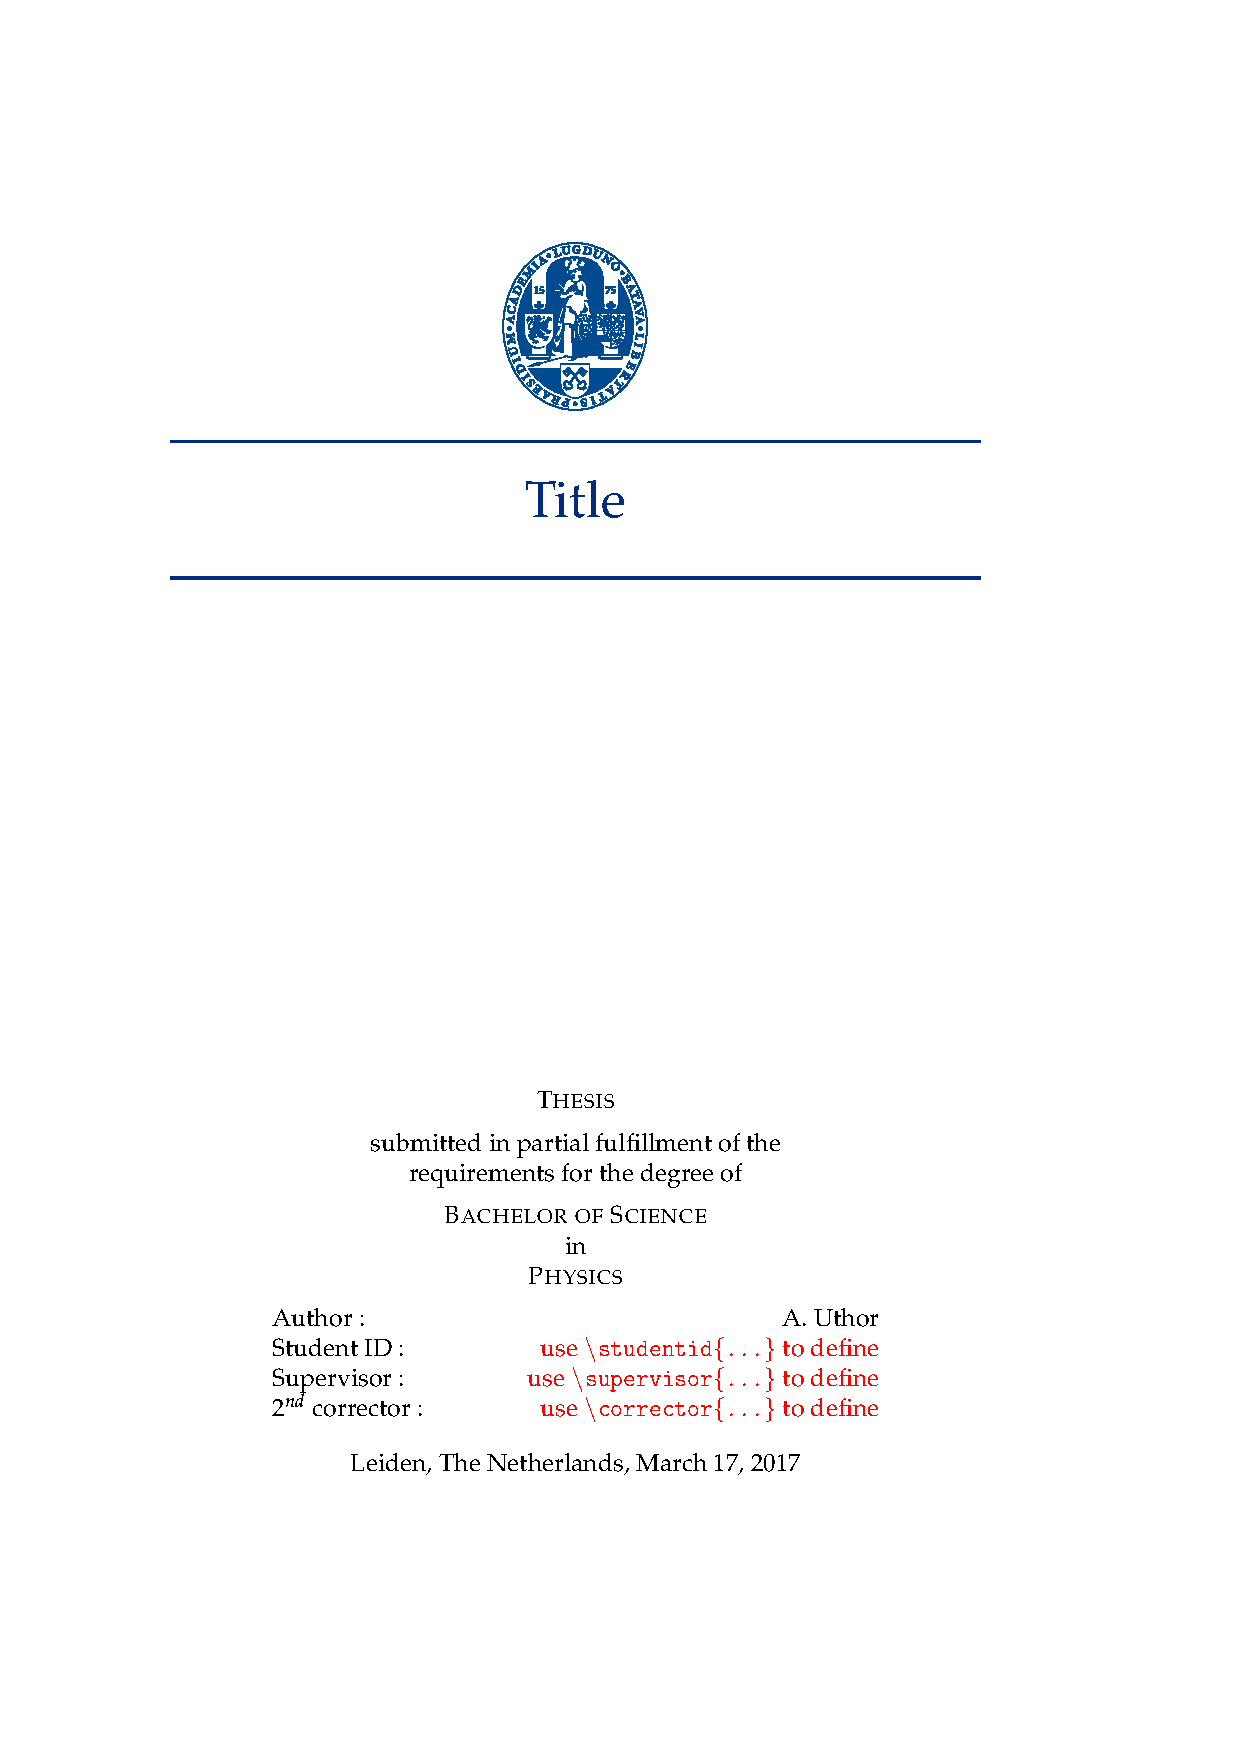
\includegraphics[scale=0.8,trim=30 300 10 40]{minimal.pdf}}
\end{center}

\section{Other Commands}
\begin{description}
\item[\texttt{\textbackslash{}bashStdout}]
After each execution of \verb+\bash+, the macro \verb+\bashStdout+
is defined to entire contents of
  the standard output of the executed script.

For example, I can write
\begin{quote}
\begin{verbatim}
To obtain the following sentence:
\bash
uname -o
\END
\begin{quote}
``This document was prepared on \emph{\bashStdout}''
\end{quote}
\end{verbatim}
\end{quote}
To obtain the following sentence:
\bash
uname -o
\END
\begin{quote}
``This document was prepared on \emph{\bashStdout}''
\end{quote}

\item[\texttt{\textbackslash{}bashStderr}]
Similar to \verb+\bashStderr+, except that it
  is defined is defined to the standard error of the executed script.
(Be ware that you must apply error tolerance flags
  to use this command, since normally,
  if the script generates anything to the standard error stream,
  \LaTeX{} processing will halt, asking for your attention.)

\item[\texttt{\textbackslash{}splice}]
Shell commands passed to the \verb+\splice+
  macro are executed in a similar fashion to
  commands enclosed between \verb+\bash+
  and \verb+\END+, but, in addition to this execution,
  \bashful incorporates the standard output into the main file.
For example, I can write 
\begin{quote}
\begin{verbatim}
Here is a nice quote for you to remember.
\begin{quote}
\emph{\splice{fortune}}
\end{quote}
\end{verbatim}
\end{quote}
To obtain
\begin{quote}
Here is a nice quote for you to remember.
\begin{quote}
\emph{\splice{fortune}}
\end{quote}
\end{quote}

Unlike the \verb+\bash+\ldots\verb+\END+,
  \verb+\splice+ does not treat its argument
  as if it was \texttt{verbatim}.
Using special characters can therefore be
  tricky with \verb+\splice+.
On the positive side, macro expansion within
  this argument can be handy.
\end{description}

\bash
cat 00.tex |\
tr -c "a-zA-Z\\\\" "\012" |\
tr "\\\\" "@" |
sed "s/@/ @/g" |\
tr " " "\012" |\
sed "/^@$/d" |\
grep @ | sort  |\
uniq -c |\
sort -n |\
awk '{print$1}' | uniq -c 
\END


	


  
\section{Customization}

\newcommand\option[3]{%
      \noindent\(
          \text{\bfseries\texttt{#1}}
          =
          \langle\text{{#2}}\rangle
      \)
      \hfill\texttt{#3}\\}
\subsection{Package Options}
Options to the \verb+\bashful+ package passed using the \textsf{xkeyval} syntax:

\option{hide}{\texttt{true}/\texttt{false}}{\texttt{false}}
If \texttt{true}, scripts are
  executed in a designated directory;
   if \texttt{false}, scrips are executed 
   in the current working directory.
   
\option{dir}{\sl directoryName}{}
If \texttt{hide} option is \texttt{true}, then
  scripts are executed in this directory.
Initial value of this options is \verb+_00+.
Note that if you use \TeX{}live 2010, you have to configure certain
  security flags to make it possible to write to directories
  whose name start with a dot, or to directories
  which are not below the current working directory.

\option{verbose}{\texttt{true}/\texttt{false}}{\texttt{false}}
If \texttt{true}, be chatty.

\option{unique}{\texttt{true}/\texttt{false}}{\texttt{false}}
If \texttt{true}, then \bashful uses  
  unique names for the files it generates in each
  invocation of the \verb+\bash+ command: \textsf{XX}\texttt{.sh}, 
  \textsf{XX}\texttt{.stdout}, \textsf{XX}\texttt{.stderr} and 
      \textsf{XX}\texttt{.exitCode}. 
These names then follow the pattern 
    \textsf{JOB}\texttt{@}\textsf{LINE}\texttt{.}\textsf{EXTENSION},
  where \textsf{JOB} is the job's name (i.e., \verb+\jobname+), 
  \textsf{LINE} is the number of the line in the input file in
  which the \verb+\bash+ command was invoked, and 
  \textsf{EXTENSION} is one of ``\texttt{sh}'', 
    ``\texttt{stdout}", ``\texttt{stderr}'' and 
      ``\texttt{exitCode}.

If \texttt{false}, then these files follow the pattern
    \textsf{JOB}\texttt{.}\textsf{EXTENSION}.

You should use this option your input invokes
  \verb+\bash+ more than once.  
    
\option{dir}{\sl directoryName}{}
If \texttt{hide} option is \texttt{true}, then
  scripts are executed in this directory.
Initial value of this options is \verb+_00+.
Note that if you use \TeX{}live, you have to configure certain
  security flags to make it possible to write to directories
  whose name start with a dot, or to directories
  which are not below the current working directory.

\subsection{Command Options}

Options to \verb+\bash+ command 
  are passed using the \textsf{xkeyval} syntax:


      

\subsubsection{File names}
\option{scriptFile}{\sl fileName}{\textbackslash jobname.sh}
Name of file into which the script instructions are spilled prior 
  to execution.
The default is \verb+\jobname.sh+; this file
  will be reused by all \verb+\bash+ commands in your documents.
  This is rarely a problem, since these scripts
  execute sequentially.

\option{stdoutFile}{\sl fileName}{\textbackslash jobname.stdout}
Name of file into which the shell standard output stream is 
  redirected. 
  

\option{stderrFile}{\sl fileName}{\textbackslash jobname.stderr}
Name of file into which the shell standard error stream is 
  redirected. 
  
\option{exitCodeFile}{\sl fileName}{\textbackslash jobname.stderr}
Name of file into which the shell standard error stream is 
  redirected. 

\subsubsection{Listing Structure}
\option{script}{\texttt{true}/\texttt{false}}{\texttt{false}}
If \texttt{true}, the content of \texttt{scriptFile} 
  is listed in the main document.

\option{stdout}{\texttt{true}/\texttt{false}}{\texttt{false}}
If \texttt{true}, the content of \texttt{stdoutFile} 
  is listed in the main document.
If both \texttt{script} and \texttt{stdout} are 
  \texttt{true}, then \texttt{scriptFile} is listed
  first, and leaving no vertical space, 
  \texttt{stdoutFile} is listed next.
  
\option{stderr}{\texttt{true}/\texttt{false}}{\texttt{false}}
If \texttt{true}, the content of \texttt{stderrFile} 
  is listed in the main document, following
  \texttt{scriptFile} (if \texttt{script} is 
  \texttt{true}) 
  and 
  \texttt{stdoutFile} (if \texttt{stdout} is 
  \texttt{true}).
  
\subsubsection{Tolerance to Errors}
\option{ignoreExitCode}{\texttt{true}/\texttt{false}}{\texttt{false}}
When
  \texttt{true} \verb+\bash+ will consider
    an execution correct even if its exit code
    is not 0.
    
\option{ignoreStderr}{\texttt{true}/\texttt{false}}{\texttt{false}}
 When \texttt{true} \verb+\bash+ will consider
    an execution correct even if produces
    output to the standard error stream.
    
\subsubsection{Appearance}
  
\option{prefix}{tokens}{\percentchar\textvisiblespace}
String that prefixes the listing of \texttt{scriptFile}. 

\option{environment}{enrionmentName}{none}
Name of \LaTeX{} environment (e.g., \texttt{quote})
  in which the listing is wrapped.
  
\subsubsection{Miscellaneous}
\option{verbose}{\texttt{true}/\texttt{false}}{\texttt{false}}
If \texttt{true}, the package logs every step it takes.

\subsection{Listings Styles}
Package 
  \href
    {ftp://ftp.tex.ac.uk/tex-archive/macros/latex/contrib/listings/listings.pdf}
    {\textsf{listing}}
  is used for all listing both the executed shell
  commands and their output.
\subsubsection{Listings Style for Script File}

Style \verb+bashfulScript+ is used for displaying the executed shell
  commands (when option \texttt{script} is used).
The current definition of this style is:
\begin{verbatim}
  \lstdefinestyle{bashfulScript}{
    basicstyle=\ttfamily,
    keywords={},
    showstringspaces=false}


\end{verbatim}
Redefine this style to match your needs.

\subsubsection{Listings Style for Standard Output}

Style \verb+bashfulStdout+ is used for displaying the output of the 
  executed shell
  commands (when option \texttt{stdout} is used).
The current definition is:
\begin{verbatim}
  % listings style for the stdoutFile, can be redefined by client
  \lstdefinestyle{bashfulStdout}{
    basicstyle=\sl\ttfamily,
    keywords={},
    showstringspaces=false
  }%

\end{verbatim}
Redefine this style to match your needs.


Style \verb+bashfulStderr+ is used for displaying the output of the 
  executed shell
  commands (when option \texttt{stderr} is used).
\begin{verbatim}
  \lstdefinestyle{bashfulStderr}{
    basicstyle=\sl\ttfamily\color{red},
    keywords={},
    showstringspaces=false
  }
\end{verbatim}
Redefine this style to match your needs.

\section{Interaction with Other Packages}
This packages tries to work around a bug in \texttt{polyglossia}
  by which \verb+\texttt+ is garbled upon 
  switching to languages which do not use the Latin alphabet.
Also, in case bidirectional \TeX{}ing is in effect,
  \bashful forces the listing to be left-to-right.


\section{History}
\begin{description}
\item[Version 0.91] Initial release.
\item[Version 0.92] 
\begin{itemize}
  \item Added \texttt{ignoreExitCode},
    \texttt{ignoreStderr}, \texttt{stderr}, 
    \texttt{exitCodeFile} command options.

 \item  
    Renamed \texttt{list} to \texttt{script}.
 \item 
    Added \texttt{hide} and \texttt{dir} package options.
\end{itemize}
\item[Version 0.93] 
\begin{itemize}
  \item Added the \texttt{unique} package flag.
  \item Added the \verb+\splice+, \verb+\bashStdout+ and \verb+\bashStderr+
				commands. 
  \item Enclosed in the packaging the Prac\TeX{} article  
				source and \texttt{.pdf} file.
\end{itemize}
\end{description}

\section{Future}
The following may get implemented some day.

\begin{enumerate}
\item \emph{A \texttt{clean} option.} This option
  will automatically erase files
  generated for storing the script, and its standard
  output and standard error streams.
  
\item \emph{A \texttt{noclobber} option.} This option
  will make this package safer, by reducing the risk
  of accidentally erasing existing files.
\end{enumerate}

\section{Acknowledgments}
The manner by which \verb+\bash+ 
  collects its arguments is based on that of
 \href
  {http://www.tn-home.de/Tobias/Soft/TeX/tobiShell.pdf}
  {\textsf{tobiShell}}.
Martin Scharrer tips on \TeX{} internals
  were invaluable.
I pay tribute to the insight and encouragement offered by Francisco Reinaldo
  which lead to the Prac\TeX{} journal publication entitled 
  \emph{Bashful Writing and Active Documents} that describes
  sophisticated applications of this package.


\appendix
\section{Source of \texttt{\jobname.sty}}
  \lstinputlisting
    [    style=input,
        basicstyle=\scriptsize\ttfamily,
        numbers=left,
        stepnumber=10,
        firstnumber=1,
        numberfirstline=true,
        numberstyle=\scriptsize\rmfamily\bfseries
    ]
    {\jobname.sty}
  
\section{Source of \texttt{\jobname.tex}}
  \lstinputlisting
    [    style=input,
        basicstyle=\scriptsize\ttfamily,
        numbers=left,
        stepnumber=10,
        firstnumber=1,
        numberfirstline=true,
        numberstyle=\scriptsize\rmfamily\bfseries
    ]
    {\jobname.tex}
\end{document}
